% id: 0256
% book: RPM 미적분Ⅱ · 02 급수
% section: 실력 Up
% figure: crop:fig-0256.png
% answer: ③
% answer_source: 답지(쪽 렌더)
% variant_level: 0 (원본 전사)
% 이 파일은 build.mjs 가 items.json 에서 만든다. 고칠 때는 items.json 을 고친다.
\smash{\raisebox{1.5mm}{\dmkichul{RPM 미적분Ⅱ 0256번 · 39쪽 · 평가원 기출}}}
그림과 같이 $\seg{A_1B_1}=4$, $\seg{A_1D_1}=1$인 직사각형~$\pt{A_1B_1C_1D_1}$에서 두 대각선의 교점을 $\pt{E_1}$이라 하자. $\seg{A_2D_1}=\seg{D_1E_1}$, $\angle\pt{A_2D_1E_1}=\dfrac{\pi}{2}$이고 선분~$\pt{D_1C_1}$과 선분~$\pt{A_2E_1}$이 만나도록 점~$\pt{A_2}$를 잡고, $\seg{B_2C_1}=\seg{C_1E_1}$, $\angle\pt{B_2C_1E_1}=\dfrac{\pi}{2}$이고 선분~$\pt{D_1C_1}$과 선분~$\pt{B_2E_1}$이 만나도록 점~$\pt{B_2}$를 잡는다. 두 삼각형~$\pt{A_2D_1E_1}$, $\pt{B_2C_1E_1}$을 그린 후 \tikz[baseline=-0.2ex]\draw[line width=0.4pt](0,0.5ex)--(0.3ex,1.6ex)--(1.3ex,-0.2ex)--cycle(2.6ex,0.5ex)--(2.3ex,1.6ex)--(1.3ex,-0.2ex)--cycle; 모양의 도형에 색칠하여 얻은 그림을 $R_1$이라 하자. 그림 $R_1$에서 $\seg{A_2B_2}:\seg{A_2D_2}=4:1$이고 선분~$\pt{D_2C_2}$가 두 선분~$\pt{A_2E_1}$, $\pt{B_2E_1}$과 만나지 않도록 직사각형~$\pt{A_2B_2C_2D_2}$를 그린다. 그림 $R_1$을 얻은 것과 같은 방법으로 세 점~$\pt{E_2}$, $\pt{A_3}$, $\pt{B_3}$을 잡고 두 삼각형~$\pt{A_3D_2E_2}$, $\pt{B_3C_2E_2}$를 그린 후 \tikz[baseline=-0.2ex]\draw[line width=0.4pt](0,0.5ex)--(0.3ex,1.6ex)--(1.3ex,-0.2ex)--cycle(2.6ex,0.5ex)--(2.3ex,1.6ex)--(1.3ex,-0.2ex)--cycle; 모양의 도형에 색칠하여 얻은 그림을 $R_2$라 하자. 이와 같은 과정을 계속하여 $n$번째 얻은 그림 $R_n$에 색칠되어 있는 부분의 넓이를 $S_n$이라 할 때, $\displaystyle\lim_{n\to\infty}S_n$의 값은?
\par\smallskip\begin{center}\setlength{\dmfigw}{227.2pt}\ifdim\dmfigw>\linewidth\setlength{\dmfigw}{\linewidth}\fi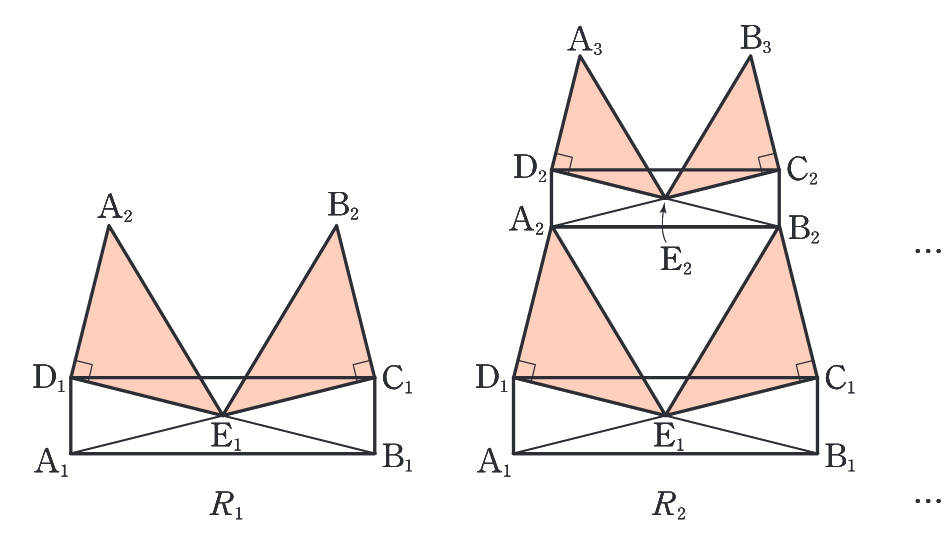
\includegraphics[width=\dmfigw]{figures/fig-0256.png}\end{center}
\begin{choices32}{\rule[-3ex]{0pt}{8ex}$\dfrac{68}{5}$}{\rule[-3ex]{0pt}{8ex}$\dfrac{34}{3}$}{\rule[-3ex]{0pt}{8ex}$\dfrac{68}{7}$}{\rule[-3ex]{0pt}{8ex}$\dfrac{17}{2}$}{\rule[-3ex]{0pt}{8ex}$\dfrac{68}{9}$}\end{choices32}
